\documentclass[conference]{IEEEtran}

\usepackage[utf8]{inputenc}
\usepackage[T1]{fontenc}
\usepackage{amsmath,amssymb,amsfonts}
\usepackage{graphicx}
\usepackage{booktabs}
\usepackage{cite}
\usepackage{xcolor}
\usepackage[hidelinks]{hyperref}

\newcommand{\nrmse}{\mathrm{NRMSE}}

\begin{document}

\title{When Classical Baselines Are Tuned as Carefully\\
as the Quantum Model, Does Quantum Reservoir\\
Computing Still Win?}

\author{\IEEEauthorblockN{Tushar Pandey}
\IEEEauthorblockA{\textit{Texas A\&M University} \\
\texttt{tusharp@tamu.edu}}}

\maketitle

\begin{abstract}
Can a small quantum computer forecast a changing signal better than an ordinary
classical method? Many studies say yes, but the classical methods they compare
against are often left in a basic, untuned state while the quantum model is
carefully optimised. We ask what happens when the classical competitor is given
exactly the same care: the same size and the same amount of tuning effort. We
study two popular reasons a quantum reservoir is thought to help, using exact
simulations of small quantum systems (up to eleven qubits) on prediction tasks.
In both cases the quantum advantage disappears once the comparison is fair. In
the first, extra quantum measurements add nothing that a simple classical formula
of the same size does not already provide. In the second, a feedback loop genuinely
helps the quantum model, turning a useless setup into a working predictor, yet a
well-tuned classical network still predicts slightly more accurately, and the gap
is statistically reliable. Our point is not that quantum reservoirs can never win,
but that two of their commonly cited advantages do not hold up against fair
classical competitors at this scale. We provide these matched comparisons as a
simple, reusable checklist for honest benchmarking. All results are fully
reproducible from fixed random seeds.
\end{abstract}

\begin{IEEEkeywords}
quantum reservoir computing, fair baselines, time-series forecasting, echo-state
networks, reproducibility
\end{IEEEkeywords}

\section{Introduction}

Reservoir computing~\cite{jaeger2001,maass2002} trains only a linear readout on
top of a fixed nonlinear dynamical system, which makes it an attractive
near-term application of quantum hardware: a fixed quantum reservoir avoids the
trainability pathologies of variational circuits~\cite{mcclean2018} while
supplying a high-dimensional nonlinear feature map. Since the original
proposals~\cite{fujii2017,nakajima2019}, a growing body of work reports that
quantum reservoir computing (QRC) outperforms classical reservoirs and recurrent
networks on chaotic, financial, and biomedical time
series~\cite{mujal2021,martinezpena2021}. At the same time, dequantization and
expressivity results~\cite{schuld2021,sweke2021} caution that the function
classes realised by such circuits can often be reproduced classically, which
makes the choice of classical baseline decisive.

A recurring weakness in these reports is the classical baseline. When a quantum
model is compared against an echo-state network (ESN)~\cite{jaeger2001} or a
polynomial readout, the strength of the conclusion depends entirely on whether
the classical model was given an equal chance: the same feature-space capacity,
the same hyperparameter-tuning budget, the same causal evaluation protocol, and a
metric that does not implicitly favour the quantum side. In practice these
conditions are often not met. Baselines are reported with default settings while
the quantum model is tuned; ``classical reservoir'' refers to a different
architecture than the quantum one; efficiency is measured as simulation
wall-clock time rather than any hardware-relevant quantity; and directional
accuracy is reported without the persistence control that makes it meaningful.

This paper asks a narrow question: \emph{when the classical baseline is matched
in capacity and tuning, does the quantum reservoir's reported advantage survive?}
We study two representative advantage mechanisms in noiseless statevector
simulation at small system size ($q\le 11$) and find that on these tasks it does
not. Our contribution is not the negative outcome per se but the two controls
that produce it: a capacity-matched classical model and a tuning-matched
classical recurrent network, together with a correctness-gated, deterministic
simulation harness. We state the scope plainly: this is a simulation study at
sizes that classical hardware can represent exactly ($q \le 11$); the claim is
``no advantage here, under fair comparison,'' not ``no advantage is possible.''

We focus on these two advantage mechanisms because they admit the cleanest
matched controls. They are part of a broader fair-comparison cartography of QRC
advantage claims, additional angles of which (high-body trajectory observables,
channel-spectrum learning, and cross-asset volatility spillover) we defer to a
companion treatment; the methodology and the two controls developed here apply to
those settings as well.

\section{Methods}
\label{sec:methods}

\subsection{Common harness and fairness controls}

All experiments share a single evaluation harness with the following properties,
several of which are the fairness controls whose absence we are critiquing.

\paragraph{Causal, leakage-free evaluation} Each series is split chronologically
into training, validation, and test segments. Every preprocessing step
(standardisation) and every hyperparameter is fit on the training/validation
portion only and applied causally; the test segment is touched once, for the
final reported number.

\paragraph{Validation-only tuning, applied equally} All free hyperparameters
(ridge penalty for every method, quantum evolution time $\tau$, feedback gain
$k_{\mathrm{fb}}$, and the ESN spectral radius and leak rate) are selected by
validation error. Importantly, the classical baselines receive the \emph{same}
tuning budget as the quantum model. This is the single most important control and
the one most often missing.

\paragraph{Matched feature dimension} Where a quantum and a classical reservoir
are compared, their readout feature dimensions are matched so that the comparison
is not confounded by readout width.

\paragraph{Correctness gates} Before any result is generated, an automated
self-test verifies: the reservoir state is physical ($\mathrm{Tr}\,\rho=1$ and
all measured expectations lie in $[-1,1]$); the two-point readout computed from
the density-matrix diagonal agrees with the explicit operator expectation to
machine precision; finite-shot estimates converge to the exact values as the shot
count grows; and, for the feedback model, that the feedback path is wired
correctly (with gain zero it reproduces the open-loop reservoir to machine
precision) and is strictly causal (perturbing a future input leaves earlier
features unchanged). Every reported number is read back from disk and checked
against a content hash; all results in this paper are deterministic and reproduce
bit-for-bit.

\paragraph{Metrics} We report normalised root-mean-square error ($\nrmse$,
normalised by the per-target standard deviation, so that $\nrmse=1$ is the
trivial mean predictor) and, for directional tasks, mean directional accuracy
(MDA). We define MDA as the fraction of test points on which the predicted
direction of the next move matches the observed direction,
$\mathrm{MDA}=\frac{1}{|\mathrm{test}|}\sum_t \mathbf{1}[\operatorname{sign}(\hat
y_{t+h}-y_t)=\operatorname{sign}(y_{t+h}-y_t)]$, where $y_t$ is the last observed
level. We report it alongside the \emph{persistence-MDA}: the same directional
accuracy achieved by the naive predictor that assumes the most recent observed
move continues ($\operatorname{sign}(y_t-y_{t-h})$). Persistence-MDA is the
meaningful floor for a directional task, since an MDA above $0.5$ is otherwise
easy to obtain on trended data.

\subsection{Quantum reservoirs}

The quantum reservoir is a fully connected transverse-field Ising system,
\begin{equation}
H = \sum_{i<j} J_{ij}\, X_i X_j + v \sum_i Z_i,
\qquad J_{ij}\sim\mathcal{U}[0,1],\ v=1,
\end{equation}
fixed after random initialisation. Classical inputs are angle-encoded via
single-qubit $R_Y$ rotations; the state evolves for time $\tau$; and the readout
consists of single-qubit expectations $\langle Z_i\rangle$ and, where indicated,
two-point correlators $\langle Z_i Z_j\rangle$, which are estimable from the same
computational-basis measurement record~\cite{huang2020}. A recurrent variant
carries memory across timesteps by partial-tracing the input qubits between
encodings, following standard recurrent-QRC constructions~\cite{nakajima2019}.
Because $Z_i$ and $Z_iZ_j$ are diagonal in the computational basis, all
correlators are obtained from the state-diagonal in a single contraction,
verified equal to the explicit operator expectation (Section~\ref{sec:methods}).

\section{Case study I: a correlator readout adds nothing beyond a
capacity-matched polynomial}
\label{sec:corr}

\subsection{Setup}

A frequently proposed route to quantum expressivity is to enrich the readout with
two-point correlators $\langle Z_i Z_j\rangle$, which capture pairwise quantum
correlations and grow the feature space quadratically. The natural question a
fair comparison must ask is whether these features carry information that an
explicit classical quadratic model does not already have.

We test this on a controlled testbed of $N=5$ coupled H\'enon maps: bounded,
genuinely quadratic, multivariate dynamics with a tunable cross-asset coupling
$c$. We compare three models on one-step prediction (all with the same windowed
ridge readout and causal protocol): the tuned correlator QRC ($q=8$, readout
tuned over $\tau$, encoding scale, and single- vs.\ two-reservoir ensemble); a
degree-2 polynomial model (\textsc{Poly2}) whose features are all pairwise
products of the windowed inputs, the \emph{capacity-matched} classical control,
given \emph{more} features than the QRC; and the concatenation
$\textsc{Poly2}\oplus\textsc{QRC}$, which tests directly whether the quantum
features add anything to the polynomial basis. Observation noise of standard
deviation $0.1$ is added so that no model can solve the map exactly through its
generating polynomial. The concatenation ablation, running the classical and
quantum feature sets together and asking whether the union beats the classical
part alone, is exactly the control omitted by typical hybrid-architecture
reports.

\subsection{Results}

Table~\ref{tab:corr} reports the verified numbers, as mean $\pm$ standard
deviation over five paired data-seed/reservoir-seed combinations per coupling.
At the one-step horizon the \textsc{Poly2} control beats the tuned QRC outright at
every coupling, and at the strongest coupling the tuned QRC degrades past the
trivial-mean predictor ($\nrmse>1$) while the classical models remain predictive.
Concatenating the quantum features onto \textsc{Poly2} changes its error only
within the seed-to-seed spread: the cat-vs-\textsc{Poly2} relative reduction is
only $\approx\!2.6\%$ at every coupling, with a standard deviation across seeds
comparable to its mean, the magnitude expected from a few extra mildly-regularising features rather
than from complementary signal. The same verdict holds on mean directional
accuracy: \textsc{Poly2} reaches $\mathrm{MDA}\approx 0.96$ (persistence $\le
0.18$), the quantum model is no better, and the concatenation does not exceed
\textsc{Poly2}. The coupling axis, which one might expect to favour the joint
quantum encoding, instead makes the QRC relatively worse (Fig.~\ref{fig:caseI}).

\begin{table}[t]
\centering
\caption{Case study I (one-step, observation noise $0.1$): correlator QRC vs.\
the capacity-matched \textsc{Poly2} control and their concatenation, on coupled
H\'enon dynamics at three couplings $c$. Values are mean $\pm$ s.d.\ over five
data-seed $\times$ reservoir-seed pairs. Lower $\nrmse$ is
better; $\nrmse<1$ is predictive. ``cat'' is $\textsc{Poly2}\oplus\textsc{QRC}$;
the final column is the relative $\nrmse$ reduction of cat over \textsc{Poly2}
(positive $=$ cat lower). Windowed feature dimensions: QRC $72$, \textsc{Poly2}
$135$, so the polynomial is given \emph{more} capacity than the quantum readout,
not less. All values verified from disk.}
\label{tab:corr}
\begin{tabular}{lcccc}
\toprule
$c$ & QRC & \textsc{Poly2} & cat & cat vs.\ \textsc{Poly2} \\
\midrule
$0.0$ & $0.726\pm0.026$ & $0.363\pm0.012$ & $0.354\pm0.012$ & $+2.6\%\pm0.3$ \\
$0.1$ & $0.766\pm0.034$ & $0.335\pm0.012$ & $0.326\pm0.007$ & $+2.6\%\pm1.5$ \\
$0.2$ & $1.030\pm0.258$ & $0.305\pm0.132$ & $0.297\pm0.125$ & $+2.7\%\pm1.0$ \\
\bottomrule
\end{tabular}
\end{table}

\begin{figure}[t]
\centering
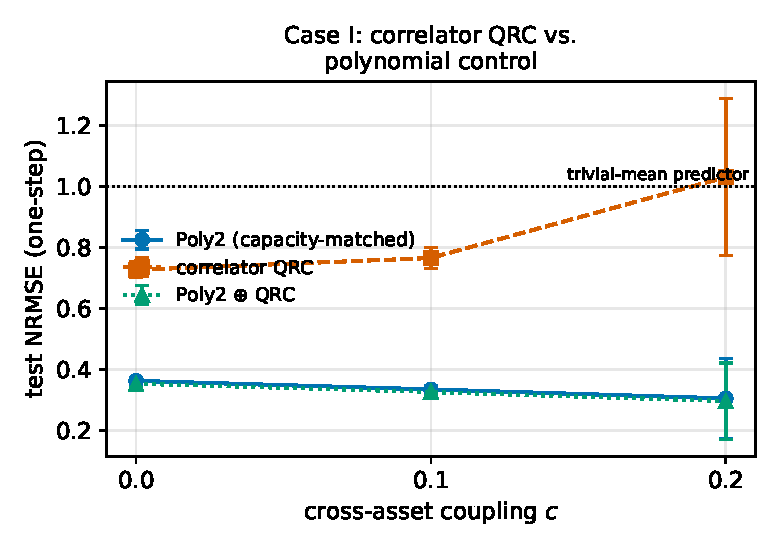
\includegraphics[width=0.92\linewidth]{fig_caseI.pdf}
\caption{Case study I. One-step test NRMSE versus cross-asset coupling $c$ for the
correlator QRC, the capacity-matched degree-2 polynomial (\textsc{Poly2}), and
their concatenation $\textsc{Poly2}\oplus\textsc{QRC}$. The polynomial control is
below the QRC at every coupling, and the concatenation tracks \textsc{Poly2}
almost exactly, so adding the quantum features changes nothing of substance. The
dotted line marks the trivial-mean predictor ($\nrmse=1$).}
\label{fig:caseI}
\end{figure}

We are precise about what this does and does not show. The coupled H\'enon
dynamics are exactly quadratic, so a degree-2 polynomial spans the true
generating function class; this is by construction the most favourable possible
setting for \textsc{Poly2}, and the result is correspondingly bounded. The claim
we make is therefore not ``a fair baseline always erases the edge,'' but the
narrower and fully supported one: \emph{when the classical model already covers
the data's function class, a two-point correlator readout contributes nothing
beyond it}. The correlator readout does help the QRC relative to a single-point
readout, but that gain does not transfer into an advantage over a classical model
of matched (indeed larger) capacity. A reader should read Case~I as a clean
refutation of the specific ``correlators add quantum expressivity'' argument on
quadratic data, not as a universal statement.

\section{Case study II: feedback is a live mechanism but loses to a
tuning-matched ESN}
\label{sec:fb}

\subsection{Setup}

A distinct advantage claim concerns \emph{feedback-driven} QRC, in which the
measurement outcome at one step modulates the reservoir drive at the next, making
the effective dynamics path-dependent rather than a fixed function of a finite
input window. Path-dependence is something a fixed-window polynomial cannot
reproduce, but it is precisely what a classical recurrent network also provides.
The honest baseline for a feedback reservoir is therefore not a polynomial but a
recurrent network, the echo-state network (ESN), and the test is whether
\emph{quantum} recurrence beats \emph{classical} recurrence at equal tuning.

We use a nonstationary task built so that recurrence is necessary: a hidden
two-state Markov process switches the sign of a first-order autoregressive
coefficient, so each regime is individually predictable but the regime must be
inferred online from the observable history. A correctness gate confirms the task
genuinely requires regime inference (an oracle given the hidden state beats a
fixed-window linear model, with the gap growing as the switching rate rises). We
implement feedback as an additive, saturating term on the input drive angle,
$\phi_t = x_t + k_{\mathrm{fb}}\tanh(\bar m_{t-1})$, where $\bar m_{t-1}$ is the
mean measurement at the previous step; $k_{\mathrm{fb}}=0$ recovers the open-loop
reservoir exactly. We compare, over ten data seeds $\times$ ten reservoir seeds
($100$ paired runs; an initial $3\times3$ grid served only as a pilot), the tuned
feedback QRC, its open-loop counterpart, a tuning-matched ESN (spectral radius
and leak rate selected on the same validation budget), \textsc{Poly2}, and a
linear model.

\subsection{Results}

Feedback is a genuine, live mechanism. In the $10\times10$-seed comparison at
$p_{\mathrm{sw}}=0.05$ (Table~\ref{tab:fb}, lower), the open-loop reservoir is
useless ($\nrmse = 1.020 \pm 0.036$, worse than the mean predictor) while closing
the loop lifts it to $0.787 \pm 0.059$, a $23\%$ improvement on identical seeds. A
single-seed switching-rate sweep (Table~\ref{tab:fb}, upper) shows the same effect
across $p_{\mathrm{sw}}\in\{0.02,0.05,0.10\}$ ($+10$ to $+19\%$); we report it as
an illustrative trend, with the load-bearing seed-averaged number taken from the
lower block. This is, to our knowledge, the clearest case in our study of a
quantum reservoir mechanism doing something its open-loop version cannot.

\begin{table}[t]
\centering
\caption{Case study II. Upper: feedback vs.\ open-loop QRC across switching rates
$p_{\mathrm{sw}}$ (single seed, illustrative). Lower: the fair test at
$p_{\mathrm{sw}}=0.05$ over $10\times10$ seeds (mean $\pm$ s.d.), one-step
$\nrmse$ and MDA (persistence MDA $=0.27$). The tuning-matched ESN beats the
feedback QRC; the paired NRMSE difference is significant ($t$-test
$p\approx10^{-21}$, Wilcoxon $p\approx10^{-16}$, bootstrap $95\%$ CI
$[0.057,0.078]$).}
\label{tab:fb}
\begin{tabular}{lccc}
\toprule
\multicolumn{4}{l}{\emph{Upper: feedback vs.\ open-loop (single seed)}}\\
$p_{\mathrm{sw}}$ & open-loop & feedback & gain \\
\midrule
$0.02$ & $1.007$ & $0.874$ & $+13.2\%$ \\
$0.05$ & $1.018$ & $0.824$ & $+19.1\%$ \\
$0.10$ & $1.032$ & $0.925$ & $+10.5\%$ \\
\midrule
\multicolumn{4}{l}{\emph{Lower: fair comparison, $10\times10$ seeds}}\\
method & $\nrmse$ & MDA & \\
\midrule
ESN (tuned)      & $0.720\pm0.060$ & $0.737\pm0.054$ & \\
Linear           & $0.750\pm0.056$ & $0.735\pm0.055$ & \\
\textsc{Poly2}   & $0.762\pm0.046$ & $0.734\pm0.055$ & \\
Feedback QRC     & $0.787\pm0.059$ & $0.728\pm0.051$ & \\
Open-loop QRC    & $1.020\pm0.036$ & $0.740\pm0.058$ & \\
\bottomrule
\end{tabular}
\end{table}

The mechanism being live, however, does not make it advantageous. Under the fair
$10\times10$-seed comparison (Table~\ref{tab:fb}, lower), the tuning-matched ESN
attains $\nrmse = 0.720 \pm 0.060$ against the feedback QRC's $0.787 \pm 0.059$,
an ESN advantage of $8.5\%$. Because the $100$ runs are paired (shared data and
reservoir seeds), we test the per-run difference directly: the mean paired
difference is $0.067$ in NRMSE (ESN better), overwhelmingly significant under both
a paired $t$-test ($t=12.3$, $p\approx1.4\times10^{-21}$) and the Wilcoxon
signed-rank test ($p\approx9\times10^{-17}$), with a bootstrap $95\%$ confidence
interval of $[0.057,\,0.078]$ that excludes zero. All three of these tests operate
\emph{across} the $100$ seeds (the across-Hamiltonian distribution): the paired
$t$- and Wilcoxon tests take the $100$ per-run ESN-minus-QRC NRMSE differences as
their sample, and the bootstrap resamples those same $100$ paired per-run
differences with replacement ($20{,}000$ resamples), so the interval reflects
across-seed/Hamiltonian variability rather than within-run test-point noise. The
ESN beats the feedback QRC in $92\%$ of the paired runs, so the result is
systematic rather than driven by a few realisations; and the feedback QRC's
spread across the $100$ reservoir/data realisations ($\mathrm{s.d.}=0.059$) is no
larger than the ESN's ($0.060$), confirming the quantum reservoir is not merely an
unlucky draw. The feedback QRC in fact trails every classical baseline, including
a plain windowed linear model ($0.750$); note that on this task the quadratic
\textsc{Poly2} features ($0.762$) are themselves worse than the linear model, a
reminder that added capacity is not automatically useful. On directional accuracy
all models cluster near $0.73$, far above the $0.27$ persistence floor but
statistically indistinguishable across methods (Fig.~\ref{fig:caseII}). The
conclusion is that quantum feedback here reconstructs the recurrent memory that a
classical recurrent network already provides, and does so slightly less
efficiently; closing the loop rescues the quantum reservoir up to, but not past,
the classical pack.

\begin{figure}[t]
\centering
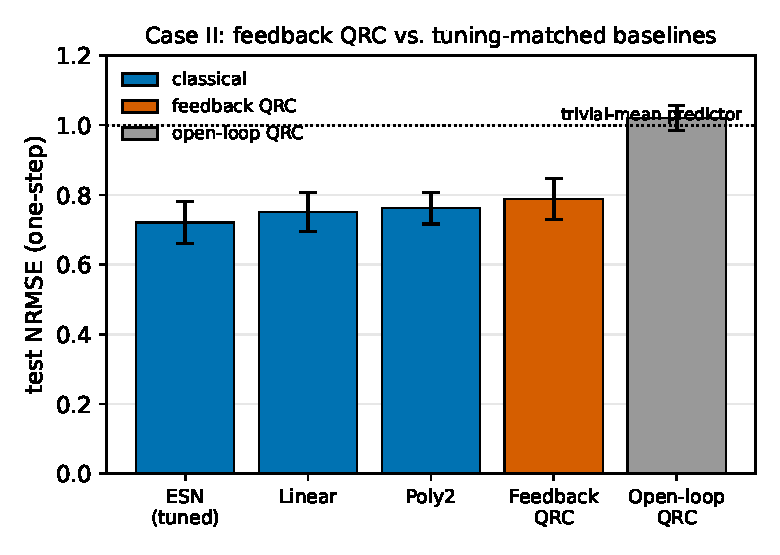
\includegraphics[width=0.92\linewidth]{fig_caseII.pdf}
\caption{Case study II. One-step test NRMSE at $p_{\mathrm{sw}}=0.05$ (mean $\pm$
s.d.\ over $10\times10$ seeds). Closing the feedback loop rescues the useless
open-loop reservoir (rightmost) to predictive performance, but the tuning-matched
ESN and even a plain linear model remain ahead of the feedback QRC. Blue bars are
classical; the dotted line is the trivial-mean predictor.}
\label{fig:caseII}
\end{figure}

\section{Discussion}

Two mechanisms, two representative advantage claims, one outcome: under a
capacity-matched classical control in the first case and a tuning-matched
classical recurrent control in the second, the quantum reservoir's reported edge
does not survive. We emphasise three points.

First, the controls are the contribution. The concatenation ablation
($\textsc{Poly2}\oplus\textsc{QRC}$ vs.\ \textsc{Poly2}) directly measures whether
quantum features add information to a classical model of matched capacity, and the
same-budget ESN measures whether quantum recurrence beats classical recurrence on
equal footing. These are inexpensive to run and clear in interpretation, yet they
are routinely omitted; including them changes the conclusion.

Second, ``live'' is not ``advantageous.'' The feedback reservoir does transform a
useless open-loop model into a predictive one. A study that compared feedback QRC
only against open-loop QRC, or against an untuned ESN, would have reported a
success. The advantage evaporates only against a classical recurrent model tuned
as hard as the quantum one.

Third, the scope is bounded and we state it as such. These are statevector
simulations at $q \le 11$, sizes a classical computer represents exactly, on tasks
with low-dimensional classical inputs. We make no claim about larger systems,
genuinely quantum-state inputs, or non-Clifford resources, where provable learning
separations are known to exist~\cite{huang2022} and the relevant comparisons may
behave differently. Our claim is the narrow, falsifiable one our experiments
support: at currently simulable scales, with fair baselines, these two QRC
advantage mechanisms do not beat their classical counterparts.

\section{Conclusion}

We have shown, under fair comparison, that two representative quantum-reservoir
advantage mechanisms, a two-point correlator readout and a feedback-driven
reservoir, do not outperform capacity- and tuning-matched classical baselines on
the tasks studied, in noiseless simulation at small scale. The two controls
behind this conclusion, a capacity-matched classical model and a same-budget
recurrent network inside a correctness-gated deterministic harness, are
inexpensive, decisive, and routinely omitted; we offer them as a reusable
template for honest QRC benchmarking rather than as a verdict on quantum reservoir
computing as a whole.

\section*{Data Availability}

The result files and the analysis scripts that generate every table and figure in
this paper are available at
\url{https://github.com/pandey-tushar/Quantum_Chaos_solver} (branch
\texttt{paper-7-cartography}). The repository includes the per-seed result JSONs
for Case~I and Case~II, the scripts (\texttt{mv\_correlator\_qrc.py},
\texttt{feedback\_qrc.py}), the figure script (\texttt{make\_figures.py}), and a
README mapping each table to the command that reproduces it. All results are
deterministic and reproduce bit-for-bit from the provided random seeds.

\begin{thebibliography}{99}

\bibitem{jaeger2001} H.~Jaeger, ``The `echo state' approach to analysing and
training recurrent neural networks,'' GMD Technical Report 148, German National
Research Center for Information Technology, 2001.

\bibitem{maass2002} W.~Maass, T.~Natschl\"ager, and H.~Markram, ``Real-time
computing without stable states: A new framework for neural computation based on
perturbations,'' \emph{Neural Comput.}, vol.~14, p.~2531, 2002.

\bibitem{mcclean2018} J.~R.~McClean, S.~Boixo, V.~N.~Smelyanskiy, R.~Babbush, and
H.~Neven, ``Barren plateaus in quantum neural network training landscapes,''
\emph{Nat. Commun.}, vol.~9, p.~4812, 2018.

\bibitem{fujii2017} K.~Fujii and K.~Nakajima, ``Harnessing disordered-ensemble
quantum dynamics for machine learning,'' \emph{Phys. Rev. Applied}, vol.~8,
p.~024030, 2017.

\bibitem{nakajima2019} K.~Nakajima, K.~Fujii, M.~Negoro, K.~Mitarai, and
M.~Kitagawa, ``Boosting computational power through spatial multiplexing in
quantum reservoir computing,'' \emph{Phys. Rev. Applied}, vol.~11, p.~034021,
2019.

\bibitem{mujal2021} P.~Mujal, R.~Mart\'inez-Pe\~na, J.~Nokkala, J.~Garc\'ia-Beni,
G.~L.~Giorgi, M.~C.~Soriano, and R.~Zambrini, ``Opportunities in quantum reservoir
computing and extreme learning machines,'' \emph{Adv. Quantum Technol.}, vol.~4,
p.~2100027, 2021.

\bibitem{martinezpena2021} R.~Mart\'inez-Pe\~na, G.~L.~Giorgi, J.~Nokkala,
M.~C.~Soriano, and R.~Zambrini, ``Dynamical phase transitions in quantum reservoir
computing,'' \emph{Phys. Rev. Lett.}, vol.~127, p.~100502, 2021.

\bibitem{schuld2021} M.~Schuld, R.~Sweke, and J.~J.~Meyer, ``Effect of data
encoding on the expressive power of variational quantum-machine-learning models,''
\emph{Phys. Rev. A}, vol.~103, p.~032430, 2021.

\bibitem{sweke2021} R.~Sweke, J.-P.~Seifert, D.~Hangleiter, and J.~Eisert, ``On
the quantum versus classical learnability of discrete distributions,''
\emph{Quantum}, vol.~5, p.~417, 2021.

\bibitem{huang2020} H.-Y.~Huang, R.~Kueng, and J.~Preskill, ``Predicting many
properties of a quantum system from very few measurements,'' \emph{Nat. Phys.},
vol.~16, p.~1050, 2020.

\bibitem{huang2022} H.-Y.~Huang, M.~Broughton, J.~Cotler, S.~Chen, J.~Li,
M.~Mohseni, H.~Neven, R.~Babbush, R.~Kueng, J.~Preskill, and J.~R.~McClean,
``Quantum advantage in learning from experiments,'' \emph{Science}, vol.~376,
p.~1182, 2022.

\end{thebibliography}

\end{document}
